\documentclass[11pt, oneside]{article} 
\usepackage{geometry}
\geometry{letterpaper} 
\usepackage{graphicx}
	
\usepackage{amssymb}
\usepackage{amsmath}
\usepackage{parskip}
\usepackage{color}
\usepackage{hyperref}

\graphicspath{{/Users/telliott_admin/Tex/png/}}
% \begin{center} 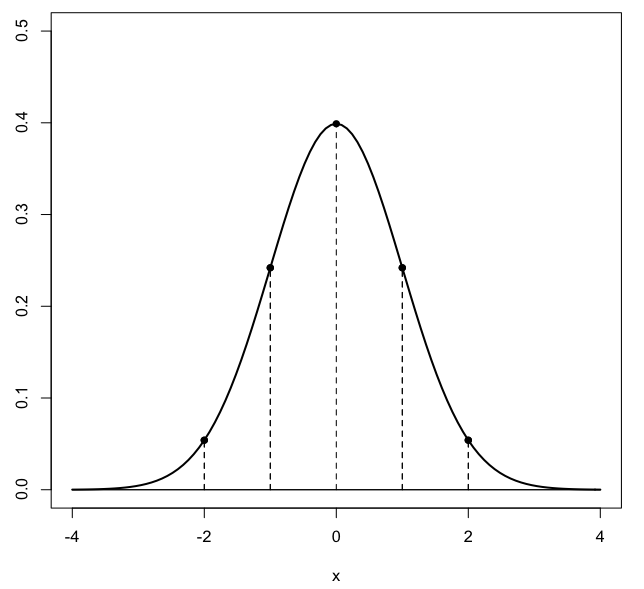
\includegraphics [scale=0.4] {gauss3.png} \end{center}

%break
\title{Revolution of a curve}
\date{}

\begin{document}
\maketitle
\Large

\subsection*{Surface area}
The next topic really is an exciting step forward in calculus.  We start looking at surface area using geometric arguments as well as results from calculus of one variable.

I will use $S$ for the surface area.  Sometimes for brevity I might write area instead of surface area.

Suppose a function $y = f(x)$ is revolved around the x-axis.  Imagine slicing it into disks in the usual way, moving along the $x$-axis in increments $dx$.  

Now, rather than compute the volume, we want the surface area of the solid.  We might try adding up the perimeter of all the disks.

Suppose we start with the simple cone with $R=H$.  The cone opens out to the right, with the vertex at the origin.  

What we have is the function
\[ y = x \]
The circumference at any point $x$ is
\[ 2 \pi y = 2 \pi x \]
And the surface area is
\[ A = \int x \ dx \]
(this has a subtle error that we will fix).
\[ = \int_0^H 2 \pi x \ dx \]
\[ = \pi x^2  \ \bigg |_0^H \]
\[ =  \pi x^2 = \pi H^2  \]
and since $H=R$
\[ =  \pi RH  \]
Now, this is obviously not the correct answer.

For the geometry, imagine cutting the surface of a cone directly along the slant and then opening the surface and laying it flat out flat.  We end up with a part (a sector) of a circle.

\begin{center} 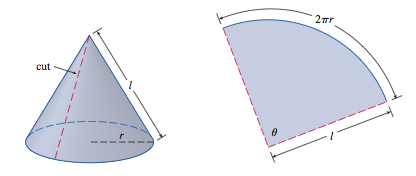
\includegraphics [scale=0.75] {cut_cone.png} \end{center}
The radius of that circle is the slant height of the cone.  The slant is labeled $l$ in the figure (not mine) and the radius is $r$.  Let's use $L$ and $R$ (capital letters for constants) in what follows:

\[ L = \sqrt{R^2 + H^2} \]
The total circumference of the circle flat in the plane would be $2 \pi L$.

However, the arc length along the sector that we actually used in the previous calculation is the circumference of the base of the cone, which is $2 \pi R$.

So the total area of the sector (equivalent to the surface area of the cone) is the total area of the circle, times the ratio of the sector circumference to the total circumference.
\[ S = \pi L^2 \ \frac{2 \pi R}{2 \pi L} = \pi RL \]

The error in our application of calculus to this problem is a factor of $L/R$, the ratio of the slant height to the radius of the base.

It turns out that what we did wrong was to multiply the circumference at each point by $dx$.  What we should have done is to multiply it by the little increment of slant instead.  This is called the path element for the curve $ds$.

Since 
\[ L = \sqrt{R^2 + H^2} \]

and in this problem
\[ R = H \]
\[ L = \sqrt{2} R \]

So the answer we obtained was $\pi R^2$, whereas the correct answer is $\pi R L$, and in this problem $L =  \sqrt{2} R$, so the correct answer is $\sqrt{2} \pi R^2$.

\subsection*{path element}

\begin{center} 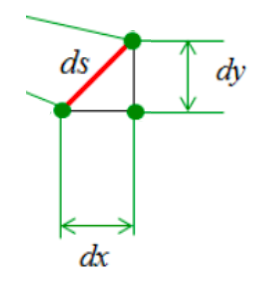
\includegraphics [scale=0.5] {path_element.png} \end{center}

For the surface area of a "volume of revolution", instead of $dx$ we need the actual length of the path element along the curve.

From Pythagoras we have 
\[ ds^2 = dx^2 + dy^2 \]
\[ = (1 + \frac{dy^2}{dx^2} ) \ dx^2 \]
\[ ds = \sqrt{1 + f'(x)^2} \cdot dx \]
We'll use this many times, both for surfaces of volumes of revolution and also for line integrals.

\subsection*{sphere:  surface area}
Calculus provides a simple proof for the surface area of a sphere, starting from the formula for the volume of a sphere
\[ V= \frac{4}{3} \pi R^3 \]

Suppose we take a sphere of radius $r$.  (I use $r$ here because now the radius will be a variable).  If we increase the radius by a little bit $dr$, then how does the volume change?  It changes exactly like the surface area!  That is
\[ dV = S \ dr \]
\[ S = \frac{d}{dr} \ V = \frac{d}{dr} \ \frac{4}{3} \pi r^3 = 4 \pi r^2 \]

Another way to see this is to break up the entire surface area of the sphere into small cones.  According to Acheson, this argument is due to Johannes Kepler.

\begin{center} 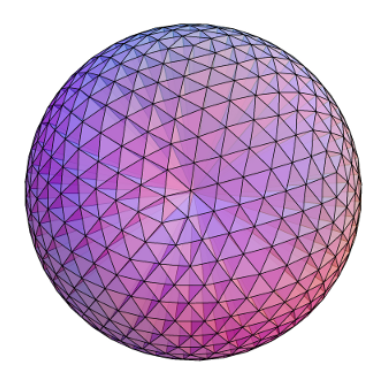
\includegraphics [scale=0.4] {sphere_area.png} \end{center}

If the number of cones is very large, the base of each one is almost flat.  Call the area of the base $dS$ and the height is  of course $R$.

The volume of a single cone is
\[ \frac{1}{3} R \ dS \]
If we add up the volumes of all the very thin cones from the entire sphere we will have the volume of the sphere
\[ \frac{1}{3}R \ S \]
but we already know this is just $4/3 \pi R^3$,
so clearly
\[ \frac{1}{3} R \cdot S = \frac{4}{3}\pi R^3 \]
\[ S = 4 \pi R^2 \]

\subsection*{slices}

Another approach is to make a volume of revolution and add up the surface part by the method of slices.  This is similar to the volume calculation we did before, except this time, for each slice we need to use the path element $ds$ rather than $dx$.

Consider a sphere of radius $R$ centered at the origin and make slices perpendicular to the $x$ axis.  We have that 
\[ y = \sqrt{R^2 - x^2} \]
The circumference for each slice is then $2 \pi y$.

When we did the volume integral for a sphere in one dimension it was
\[ V = \int_{-R}^{R} \pi y^2 \ dx \]

Here we are looking for the surface area, and adding up a bunch of small strips from the perimeter, but the differential is not $dx$  In other words, we can't just do
\[ S = \int  2 \pi y \ dx \]

For the surface area of a "volume of revolution", instead of $dx$ we need the actual length of the path element along the curve. 
\[ ds = \sqrt{1 + f'(x)^2} \cdot dx \]

What is the slope of a circle?
\[ y = \sqrt{R^2 - x^2} \]
\[ \frac{dy}{dx} = f'(x) = -\frac{x}{\sqrt{R^2 - x^2}}  = -\frac{x}{y}  \]
so
\[ ds = \sqrt{1 + f'(x)^2} \cdot dx \]
\[ = \sqrt{1 + \frac{x^2}{y^2}} \ dx \]

We want
\[ S = \int  2 \pi y \ ds \]
\[ = \int  2 \pi y \ \sqrt{1 + \frac{x^2}{y^2}} \ dx  \]
\[ = 2 \pi \int \sqrt{y^2 + x^2} \ dx \]
\[ = 2 \pi R \int \ dx \]
\[ = 2 \pi R \ x \ \bigg |_{-R}^R = 4 \pi R^2 \]

That simplified beautifully.  Usually integrals with the path element get messy.

\subsection*{Gabriel's horn}

The inverse function is 
\[ f(x) = \frac{1}{x} \]
\[ f'(x) = -\frac{1}{x^2} \]

\begin{center} 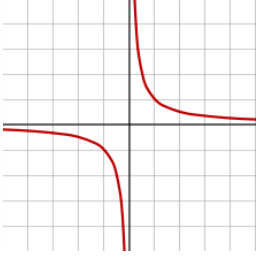
\includegraphics [scale=0.5] {inverse.png} \end{center}

We consider the curve from $x = 1 \rightarrow \infty$.

To get the surface area
\[ S = \int 2 \pi y \ ds \]
\[ = 2 \pi \int \frac{1}{x} \ \sqrt{1 + f'(x)^2} \ dx \]
\[ = 2 \pi \int \frac{1}{x} \ \sqrt{1 + \frac{1}{x^4}} \ dx \]

This looks hard!  However, we notice that the factor 
\[  \sqrt{1 + \frac{1}{x^4} } > 1 \]

So, if the integral without this factor diverges, the one with it diverges too.  And
\[ \int_1^{\infty} \frac{1}{x}\ dx = \ln x \ \bigg |_1^{\infty}  \]
certainly diverges at the upper limit.

\begin{center} 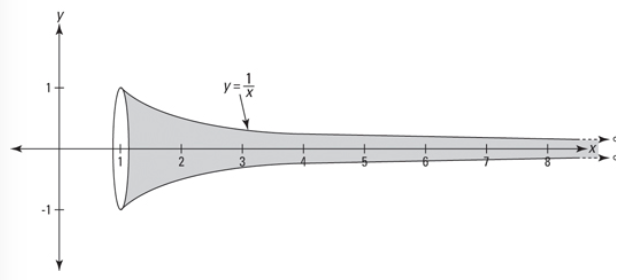
\includegraphics [scale=0.5] {gabriel_horn.png} \end{center}
Why is it so surprising that the surface area of this horn is infinite?  It is surprising because the volume is finite.

The volume is
\[ \int \pi y^2 \ dx \]
\[ = \int \pi \frac{1}{x^2} \ dx \]
\[ = \pi \ [ - \frac{1}{x}  \ \bigg |_1^{\infty}  ]  = \pi \]
Wait for the inevitable joke:  doesn't that blow your mind?

\subsection*{Volumes}

\label{sec:Volumes_of_revolution}

A solid of revolution is formed by revolving a curve around a central axis, typically, the $x$-axis.  We can get the volume of the solid by slicing it into disks.

In \hyperref[sec:Sphere_and_cone]{\textbf{Sphere and cone}}, we revolved a half-circle to obtain the volume of a sphere.  The integral was
\[ V = \int_{-R}^{R} \pi y^2 \ dx \]

We also did the cone:
\[ V = \pi \int_0^H ( \frac{R}{H} x)^2 \ dx \]

However, this approach can be used with any curve or pair of curves.

We also found just above, the volume (and surface area) of Gabriel's horn, using the curve $y = 1/x$.

The volume of the solid formed by rotating the curves $f(x)$ and $g(x)$ around the $x$-axis on the interval $[a,b]$ ($f(x) < g(x)$ everywhere) is:
\[ V = \int_a^b f(x)^2 - g(x)^2 \ dx \]

For $g(x) = 0$ this resolves to the familiar form.

If the curve is given in parametric form (both $x$ and $y$ as a function of $t$), then

\[ V_x = \int_a^b \pi y^2 \ \frac{dx}{dt} \ dt \]
\[ V_y = \int_a^b \pi x^2 \ \frac{dy}{dt} \ dt \]

where $V_x$ is revolved around the $x$-axis, and so on.

The corresponding surface areas are

\[ A_x = \int_a^b 2 \pi y \ \sqrt{(\frac{dx}{dt})^2 + (\frac{dy}{dt})^2} \ dt \]
\[ A_y = \int_a^b 2 \pi x \ \sqrt{(\frac{dx}{dt})^2 + (\frac{dy}{dt})^2} \ dt \]

\subsection*{Torus}
Consider a circle of radius $R$, displaced upward from the $x$-axis.  The distance from the origin to the center of the circle is $a$.

The equation of the upper half of this circle is
\[ y = \sqrt{R^2 - x^2} + a  \]
So
\[ y^2 = R^2 - x^2 + a^2 + 2 a \sqrt{R^2 - x^2} \]

The equation of the bottom half of the circle is almost identical
\[ y  = -\sqrt{R^2 - x^2} + a  \]
So
\[ y^2 = R^2 - x^2 + a^2 - 2 a \sqrt{R^2 - x^2} \]

Subtracting the bottom from the top, the first three terms cancel and we have
\[ y_{\text{top}}^2 - y_{\text{bottom}}^2 = 4 a \sqrt{R^2 - x^2} \]
Don't forget to multiply by $\pi$:
\[ A = 4 \pi a \sqrt{R^2 - x^2} \]

Adding up the area of each slice of the donut
\[ V = \int_{-R}^{R} 4 \pi a \sqrt{R^2 - x^2} \ dx \]

We need a trig substitution:
\[ x = R \sin t \]
\[ dx = R \cos t \ dt \]
\[ \sqrt{R^2 - x^2} = R \cos t \]
So the integral is $4 \pi a$ times
\[ R^2 \int \cos^2 t \ dt \]

As always:
\[ \int \cos^2 t \ dt = \frac{1}{2} \ [ t + \sin t \cos t \ ]  \]
And if the bounds are right, that second term will disappear.  Let's see.
\[ x = [-R,R] \]
\[ t = [-\pi/2,\pi/2] \]
The second term does go away, giving $\pi$ for what's in the brackets, and we obtain finally
\[ V = 4 \pi a \cdot R^2 \cdot \frac{\pi}{2} \]
\[ = 2 \pi a \cdot \pi R^2 \]

This is the same as obtained by multiplying the area of the cross-section of the torus by the distance traveled by the center in revolving around the $x$-axis.  The general principle is named after Pappus.

\end{document}